% =====================================================================
% FIGURES — uploaded as a SEPARATE file at initial submission.
%
% RSNA: "For new submissions, figure legends should appear directly after the
% relevant figure in the combined figure text document." So each figure here is
% immediately followed by its legend, in text-citation order. The same legends
% also appear collectively in the Figure Legends section of main.tex.
%
% AT REVISION this file is replaced by individual production-quality image
% files, one per figure (and one per panel of a multipart figure), named
% "Figure 1.tif", "Figure 6a.tif", etc.:
%   - photographic/clinical images: PSD, TIF, AI or EPS at 300 dpi. PNG is NOT
%     accepted, so figures 1 and 6 must be re-exported.
%   - graphs and line art: PSD, TIF, PPT, AI or EPS at 1200 dpi, layers retained.
% The matplotlib figures should be regenerated with savefig(..., format="tif",
% dpi=1200) rather than upscaled from the existing PNGs.
% =====================================================================
\documentclass[11pt]{article}
\usepackage[margin=1in]{geometry}
\usepackage{graphicx}
\usepackage{float}
\usepackage{setspace}
\usepackage{times}
\graphicspath{{../figures/}}
\doublespacing
\raggedright
\pagestyle{empty}
\setlength{\parindent}{0pt}
\setlength{\parskip}{0.6em}

\begin{document}

\begin{center}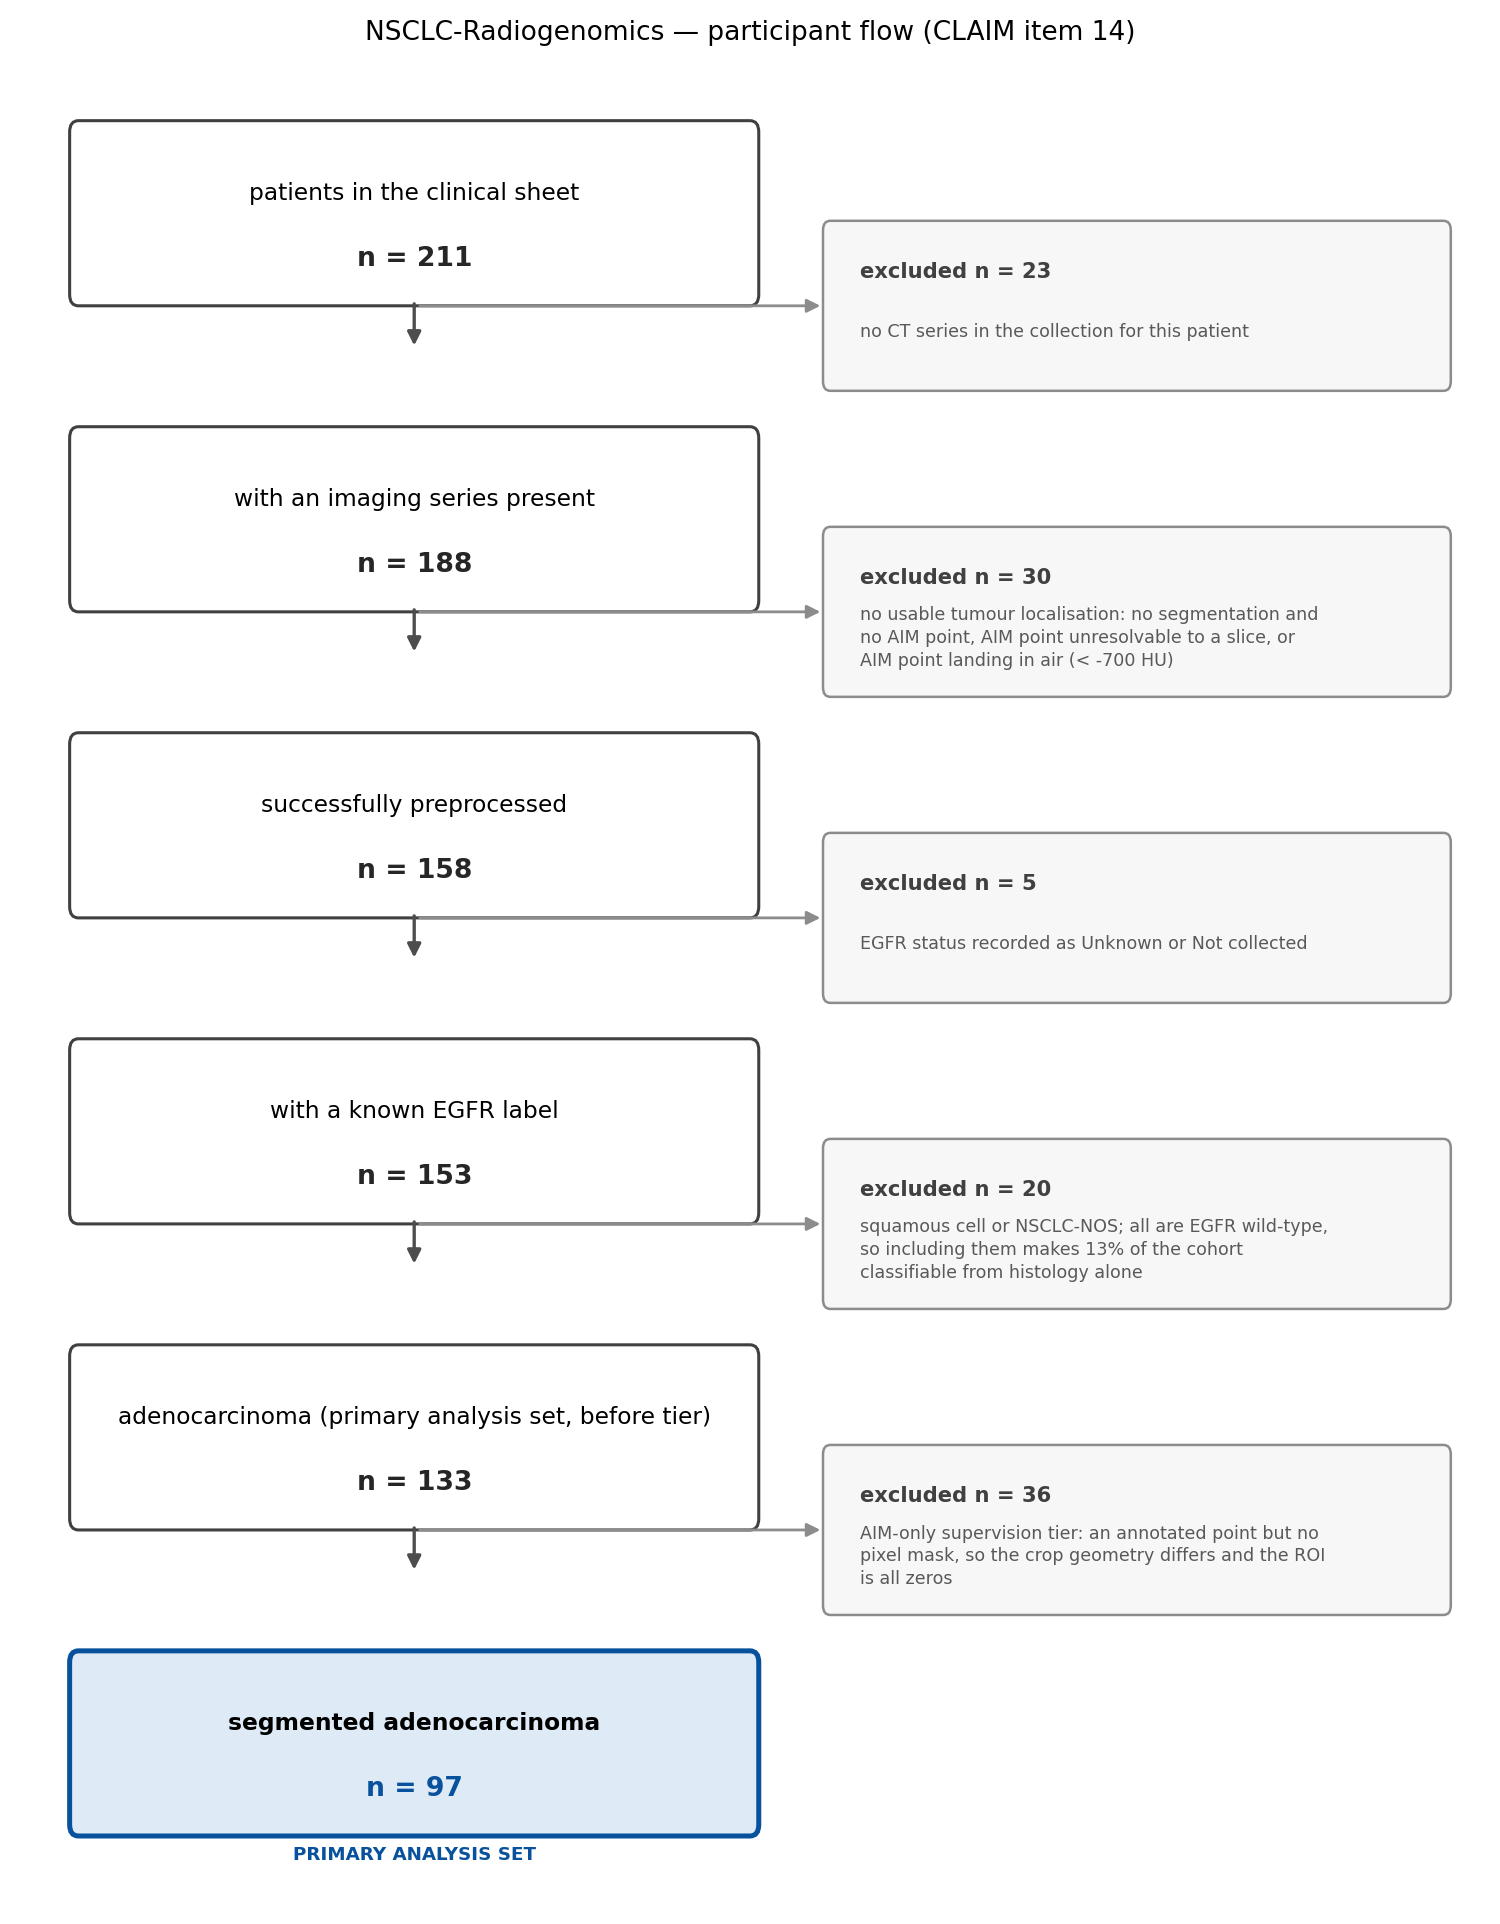
\includegraphics[width=0.72\textwidth]{fig1_flow.png}\end{center}

\textbf{Figure 1:} Flowchart shows participant flow through the study. Counts and
exclusion reasons are generated from the analysis pipeline rather than
transcribed, and reconcile exactly ($211 - 114 = 97$). The pre-specified primary
analysis set is patients with segmented adenocarcinoma.
\textit{EGFR} = epidermal growth factor receptor, NSCLC = non--small cell lung
cancer.

\clearpage
\begin{center}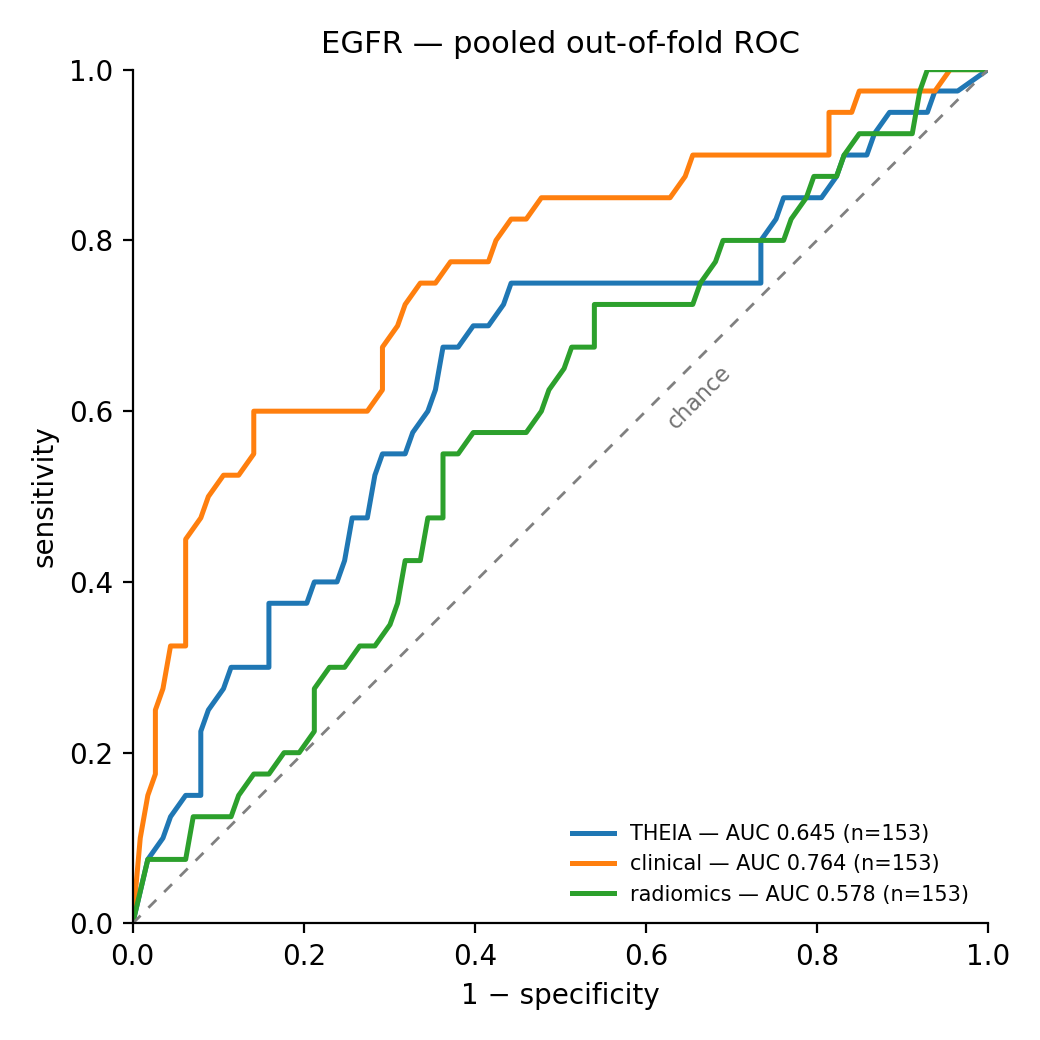
\includegraphics[width=0.62\textwidth]{fig1_roc.png}\end{center}

\textbf{Figure 2:} Graph shows pooled out-of-fold receiver operating
characteristic curves by arm, computed on identical patients and folds. The
chance line is drawn and labeled, and each arm's number of patients is printed
because the arms do not all cover the same patients.
AUC = area under the receiver operating characteristic curve.

\clearpage
\begin{center}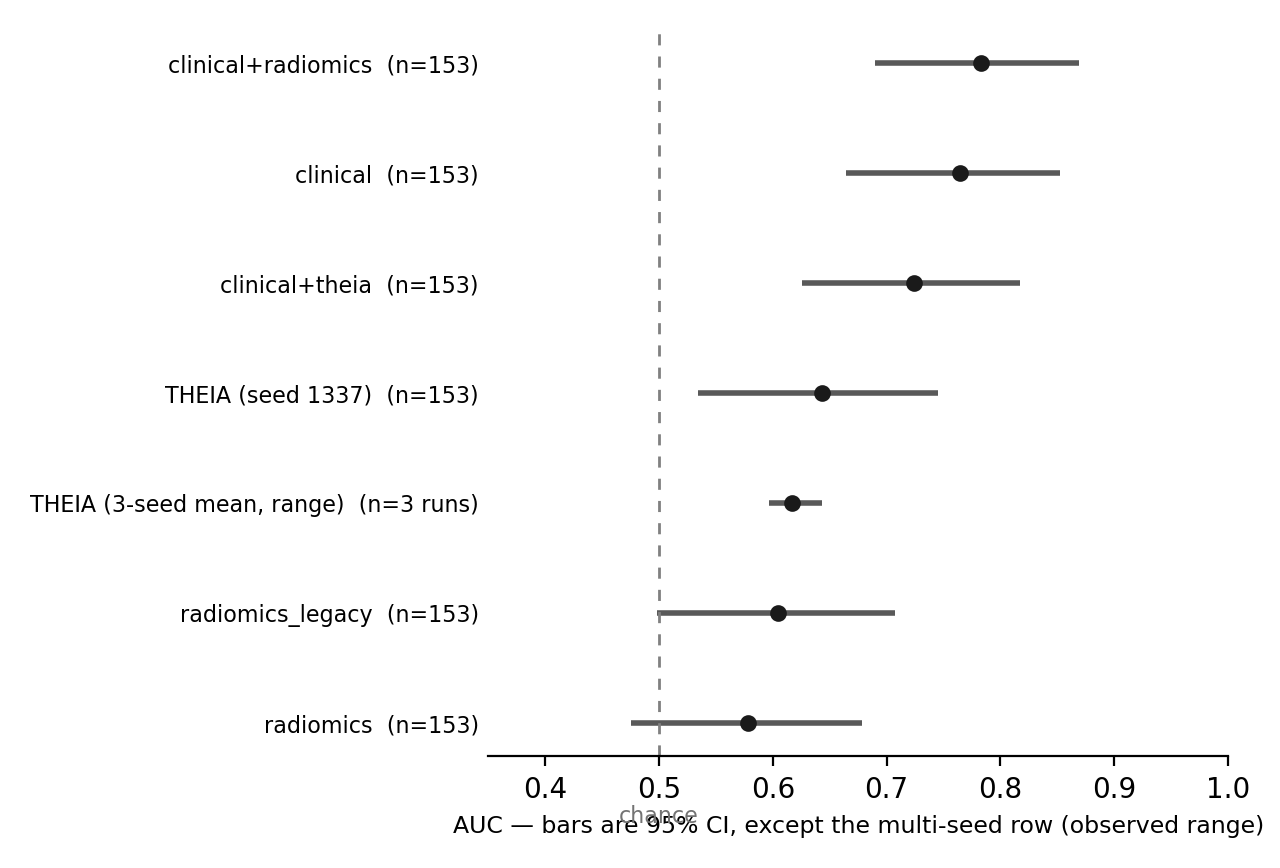
\includegraphics[width=0.86\textwidth]{fig2_forest.png}\end{center}

\textbf{Figure 3:} Forest plot shows every arm with its 95\% confidence interval.
Overlapping intervals can still differ significantly when the comparison is
paired, which is why the paired differences are reported alongside.
AUC = area under the receiver operating characteristic curve,
CI = confidence interval.

\clearpage
\begin{center}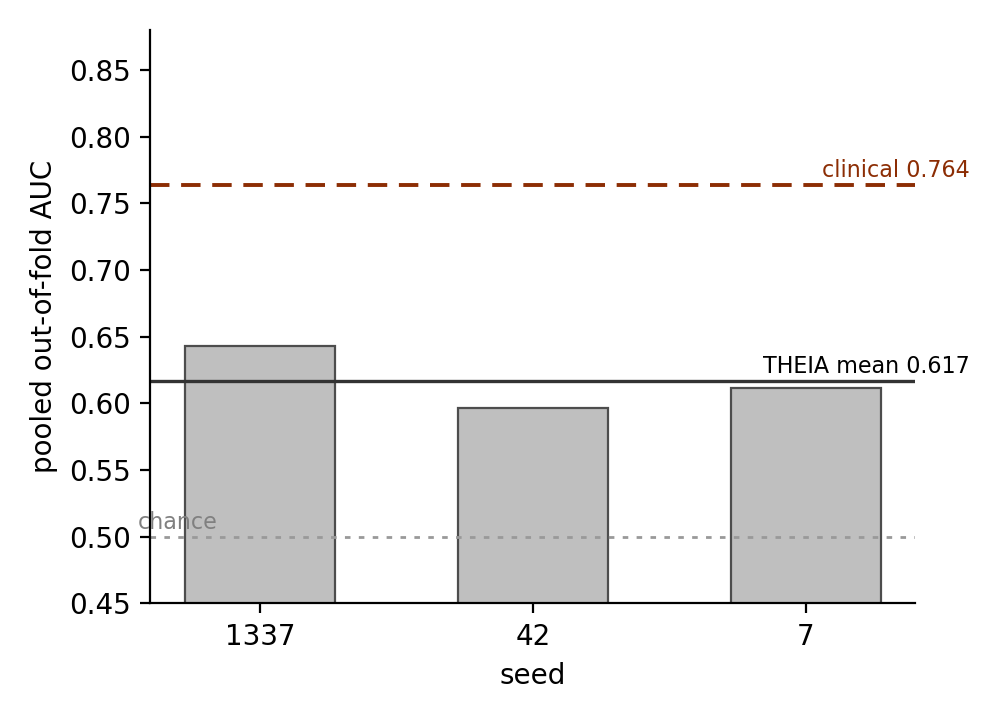
\includegraphics[width=0.62\textwidth]{fig3_seeds.png}\end{center}

\textbf{Figure 4:} Graph shows per-seed area under the receiver operating
characteristic curve against the clinical baseline. The rerun spread is shown next
to the effect being claimed; the gap to a five-variable clinical model exceeds it.
AUC = area under the receiver operating characteristic curve.

\clearpage
\begin{center}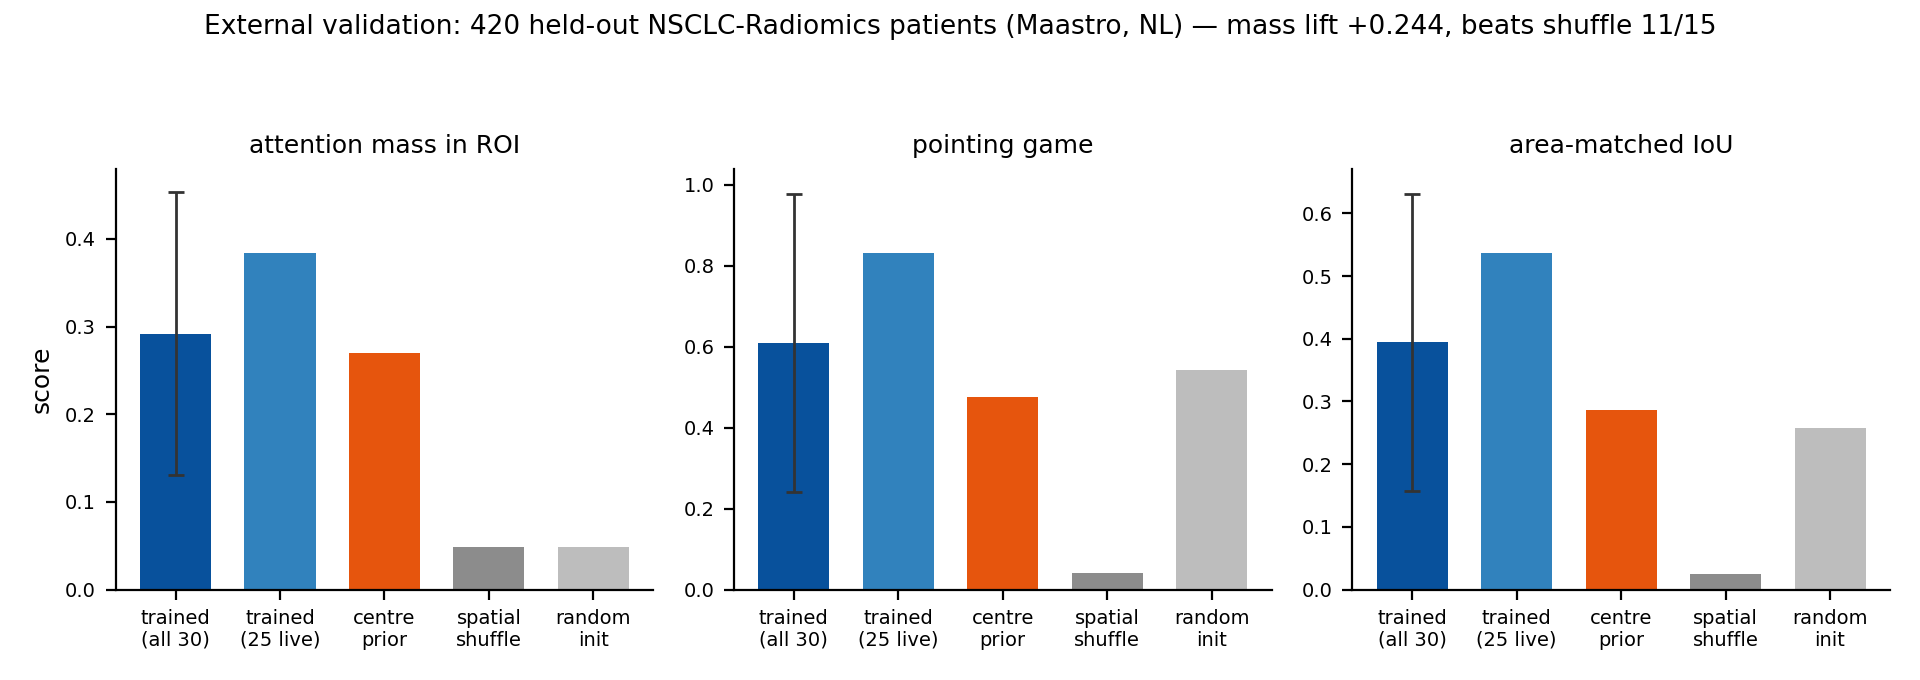
\includegraphics[width=\textwidth]{fig6_external_grounding.png}\end{center}

\textbf{Figure 5:} Graphs show the primary endpoint --- localization on 420
held-out NSCLC-Radiomics patients --- with all three controls in every panel. The
center prior is strong on attention mass by construction and weak on pointing
accuracy and area-matched intersection over union, which are invariant to its
width, so the trained model's margin is read from the right-hand panels rather
than the left. IoU = intersection over union,
NSCLC = non--small cell lung cancer.

\clearpage
\begin{center}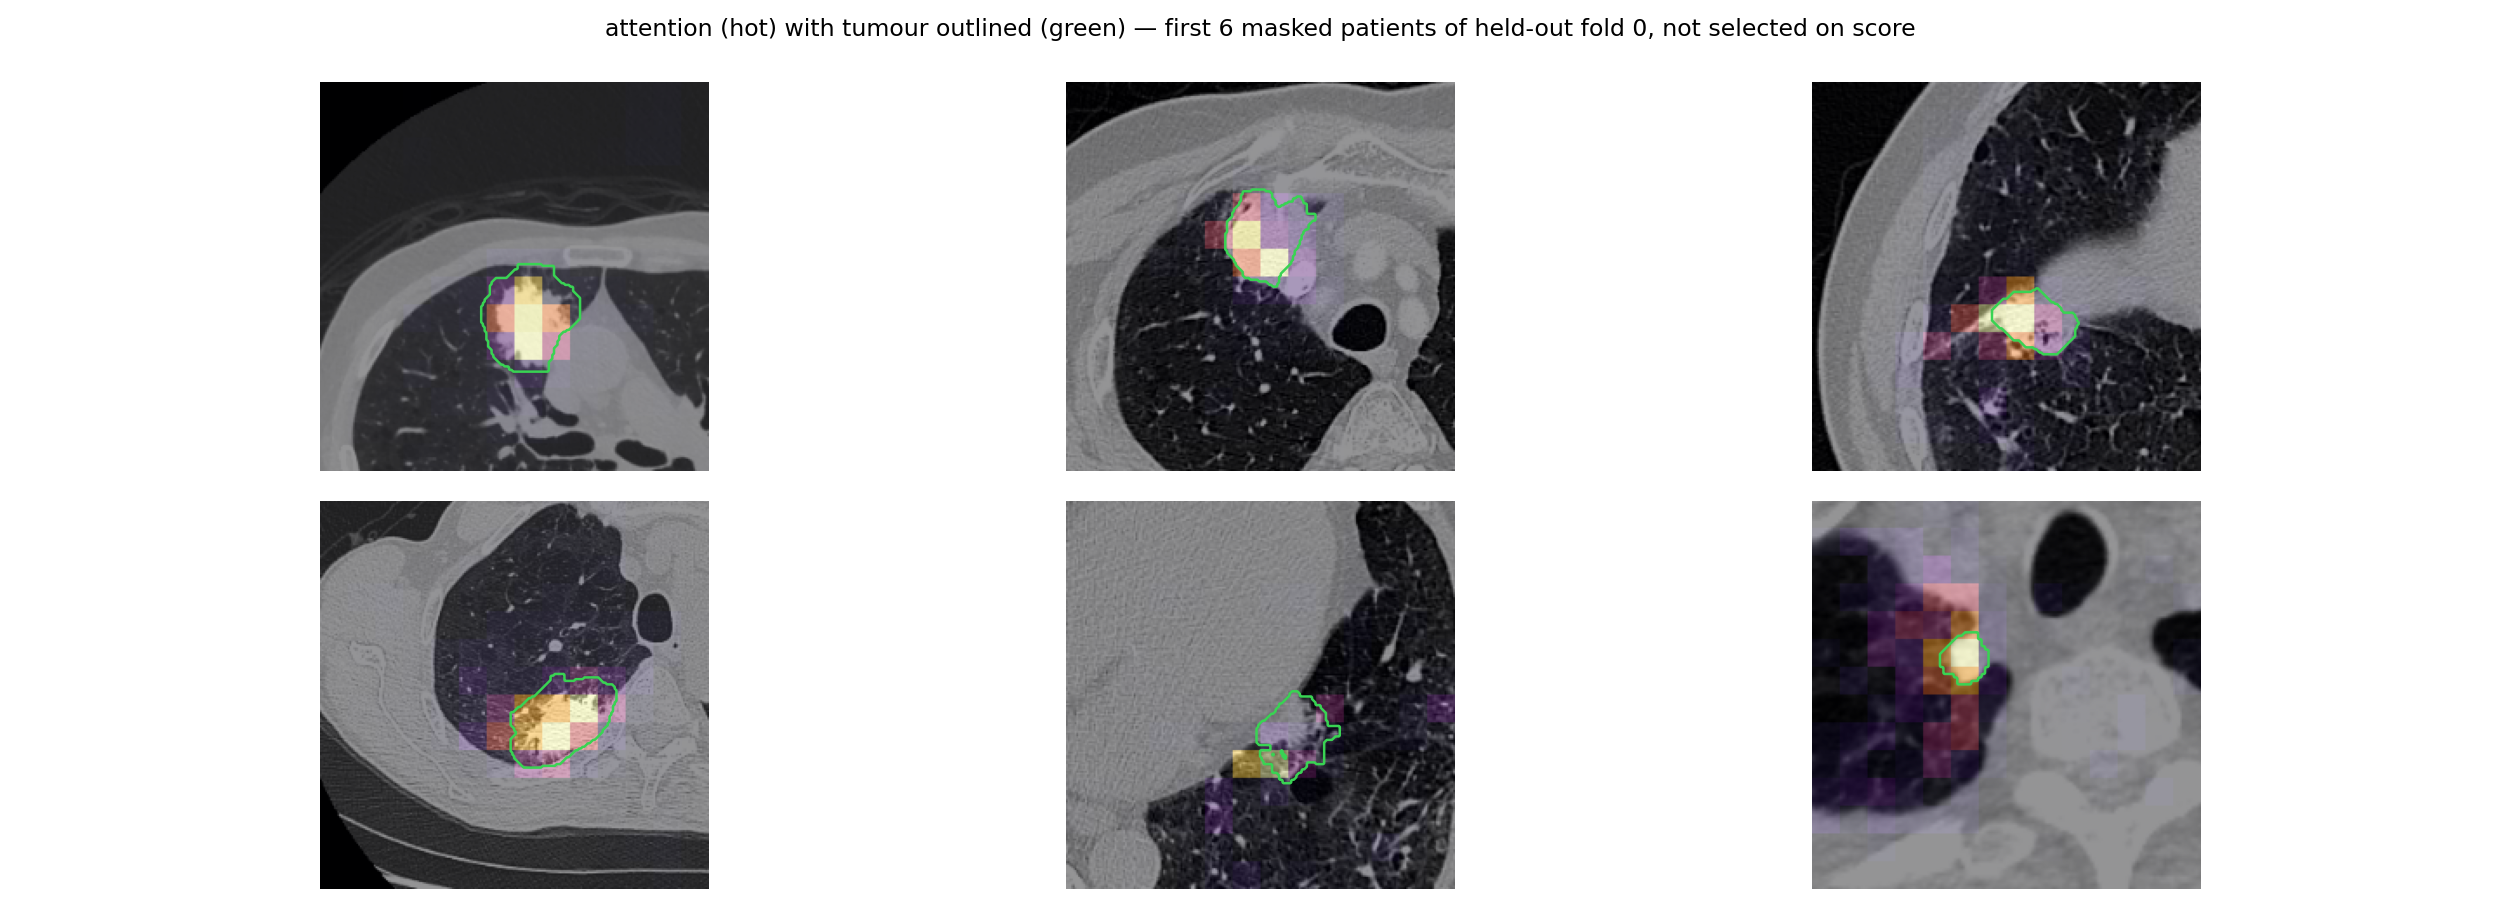
\includegraphics[width=\textwidth]{fig5_overlays.png}\end{center}

\textbf{Figure 6:} CT images with superimposed attention maps (hot colors) and the
tumor contour drawn from the reference segmentation (green) in six patients:
(A) 68-year-old man with adenocarcinoma, (B) 76-year-old man with NSCLC not
otherwise specified, (C) 64-year-old man with NSCLC not otherwise specified,
(D) 63-year-old man with adenocarcinoma, (E) 84-year-old man with adenocarcinoma,
and (F) 59-year-old man with squamous cell carcinoma. These are the first six
patients with a segmentation, in index order, from held-out fold 0 of training run
B in Table 3; they were not selected on score, and the histologic mix is whatever
that rule produced. Images are from the NSCLC-Radiogenomics collection, used under
its CC BY 3.0 license (9). NSCLC = non--small cell lung cancer.

\end{document}
